
\section{Higher-Order Model Boundary Conditions}
\label{sc:higher-order-bcs}

We now carry out an approximate derivation of the boundary conditions that are implemented with CISM's higher-order scheme. By approximate we mean that some of the derivation is guided by physical intuition and reasonable arguments, rather than rigorous mathematics. In the end, we derive the same set of equations as when following the more rigorous approach (see, e.g. \citet{DUKOWICZ:2010wb}). We will look at the derivation in three parts, (1) the free surface boundary condition, (2) the basal traction boundary condition, and (3) lateral boundary conditions.

\subsection{Stress-free Surface}
At the upper ice surface, a stress-free boundary condition is applied. The traction vector $T_i$ must be continuous across the ice sheet surface and, assuming that atmospheric pressure and surface tension are small, we have

\begin{equation}
  \label{ho.eq.surface_traction}
  \begin{split}
    & T_{i} = -T_{i(\textrm{boundary})}\approx 0, \\ 
    & T_{i} = \sigma _{ij}n_{j} = \sigma _{i1}n_{1} + \sigma _{i2}n_{2} + \sigma _{i3}n_{3} = 0, \\
  \end{split}
\end{equation}

\noindent
where the $n_i$ are the components of the outward facing, unit normal vector in Cartesian coordinates.

For a function \textit{F(x,y,z) = z -- f(x,y) = 0}, where \textit{z = f(x,y)} defines the surface, the gradient of \textit{F(x,y,z)} gives the components of the surface normal vector. For the case of the ice sheet surface, $s = f(x,y)$ and the surface normal is given by

\begin{equation}
  n_{i}=\left( -\frac{\partial s}{\partial x},-\frac{\partial s}{\partial y},1 \right)\frac{1}{a},
\end{equation}

\noindent
where

\begin{equation}
  a = \sqrt{\left( \frac{\partial s}{\partial x} \right)^{2} + \left( \frac{\partial s}{\partial y} \right)^{2} + 1}.
\end{equation}

\noindent
Eq. \eqref{ho.eq.surface_traction} gives three equations that must be satisfied at the free surface:

\begin{equation}
  \begin{split}
    & i=x: \quad T_{x} = \sigma _{xx}n_{x} + \sigma _{xy}n_{y} + \sigma _{xz}n_{z}=0, \\ 
    & i=y: \quad T_{y} = \sigma _{yx}n_{x} + \sigma _{yy}n_{y} + \sigma _{yz}n_{z}=0, \\ 
    & i=z: \quad T_{z} = \sigma _{zx}n_{x} + \sigma _{zy}n_{y} + \sigma _{zz}n_{z}=0. \\ 
  \end{split}
\end{equation}

\noindent
Expanding the $z$ equation and expressing stresses in terms of strain rates and pressures, where $\eta$ is the effective viscosity defined above, gives

\begin{equation}
  \left( 2\eta \dot{\varepsilon }_{zx} \right)n_{x}+\left( 2\eta \dot{\varepsilon }_{zy} \right)n_{y}+\left( 2\eta \dot{\varepsilon }_{zz}-P \right)n_{z}=0.
\end{equation}

\noindent
Solving for the pressure gives

\begin{equation}
  Pn_{z} = \left( 2\eta \dot{\varepsilon }_{zz} \right)n_{z}+\left( 2\eta \dot{\varepsilon }_{zx} \right)n_{x}+\left( 2\eta \dot{\varepsilon }_{zy} \right)n_{y}.
\end{equation}

\noindent
Expanding in terms of velocity gradients and normal vector components, we find

\begin{equation}
  P = 2\eta \frac{\partial w}{\partial z}-\left( \eta \frac{\partial u}{\partial z} \right)\frac{\partial s}{\partial x}-\left( \eta \frac{\partial v}{\partial z} \right)\frac{\partial s}{\partial y},
\end{equation}

where we have made the usual first-order approximation that 

\begin{equation}
  \frac{\partial w}{\partial x}=\frac{\partial w}{\partial y}\approx 0.
\end{equation}

\noindent
\textit{(WHL: and also assumed $a \approx 1$?)}

\textbf{WHL: The rest of this section derives BC discretizations that were used in Glam but are not necessary
in a finite-element approach. So I think the remaining text could be rewritten a bit and considerably shortened.}

We use this expression for the pressure and expand the two horizontal boundary condition expressions

\begin{equation}
\begin{split}
 & i=x:\quad T_{x}=\sigma _{xx}n_{x}+\sigma _{xy}n_{y}+\sigma _{xz}n_{z}=0, \\ 
 & i=y:\quad T_{y}=\sigma _{yx}n_{x}+\sigma _{yy}n_{y}+\sigma _{yz}n_{z}=0, \\
\end{split}
 \end{equation}

in terms of velocity gradients and the effective viscosity to obtain

\begin{equation}
\begin{split}
   {} & \hat{x}:\quad -2\eta \frac{\partial u}{\partial x}\frac{\partial s}{\partial x}-\eta \left( \frac{\partial u}{\partial y}+\frac{\partial v}{\partial x} \right)\frac{\partial s}{\partial y}+\eta \frac{\partial u}{\partial z}=  \\
   {} & \quad \quad \quad \quad \quad -2\eta \frac{\partial w}{\partial z}\frac{\partial s}{\partial x}+\eta \frac{\partial u}{\partial z}\left[ \frac{\partial s}{\partial x}\frac{\partial s}{\partial x} \right]+\eta \frac{\partial v}{\partial z}\left[ \frac{\partial s}{\partial y}\frac{\partial s}{\partial x} \right],  \\
%\end{equation}
%
%\begin{equation}
   {} & \hat{y}:\quad -2\eta \frac{\partial v}{\partial y}\frac{\partial s}{\partial y}-\eta \left( \frac{\partial u}{\partial y}+\frac{\partial v}{\partial x} \right)\frac{\partial s}{\partial x}+\eta \frac{\partial v}{\partial z}=  \\
   {} & \quad \quad \quad \quad \quad -2\eta \frac{\partial w}{\partial z}\frac{\partial s}{\partial y}+\eta \frac{\partial u}{\partial z}\left[ \frac{\partial s}{\partial x}\frac{\partial s}{\partial y} \right]+\eta \frac{\partial v}{\partial z}\left[ \frac{\partial s}{\partial y}\frac{\partial s}{\partial y} \right].  \\
\end{split}
\end{equation}

In both of these expression, the terms in square brackets are $\sim{0}$ (because slopes on ice sheets are small and the slope squared is exceedingly small). From continuity, we also have

\begin{equation}
\frac{\partial w}{\partial z}=-\frac{\partial u}{\partial x}-\frac{\partial v}{\partial y}.
\end{equation}

Using this expression for the normal vertical velocity gradient and removing the terms in square brackets our two horizontal boundary condition expressions become

\begin{equation}
\begin{split}
   {} & \hat{x}:\quad -2\eta \frac{\partial u}{\partial x}\frac{\partial s}{\partial x}-\eta \left( \frac{\partial u}{\partial y}+\frac{\partial v}{\partial x} \right)\frac{\partial s}{\partial y}+\eta \frac{\partial u}{\partial z}=2\eta \left( \frac{\partial u}{\partial x}\frac{\partial s}{\partial x}+\frac{\partial v}{\partial y}\frac{\partial s}{\partial x} \right),  \\
   {} & \hat{y}:\quad -2\eta \frac{\partial v}{\partial y}\frac{\partial s}{\partial y}-\eta \left( \frac{\partial u}{\partial y}+\frac{\partial v}{\partial x} \right)\frac{\partial s}{\partial x}+\eta \frac{\partial v}{\partial z}=2\eta \left( \frac{\partial u}{\partial x}\frac{\partial s}{\partial y}+\frac{\partial v}{\partial y}\frac{\partial s}{\partial y} \right).  \\
\end{split}
\end{equation}

%As in the derivation of the 1st-order stress balance equations, collect terms of a particular velocity gradient (that is, \textit{u} or \textit{v}) and move them to one side of the equation 
Moving terms to one side and dividing through by the effective viscosity \textit{\(\eta{}\)}, we arrive at the final form of the 1st-order, free surface boundary conditions

\begin{equation}
\begin{split}
   {} & \hat{x}:\quad 4\frac{\partial u}{\partial x}\frac{\partial s}{\partial x}+\frac{\partial u}{\partial y}\frac{\partial s}{\partial y}+2\frac{\partial v}{\partial y}\frac{\partial s}{\partial x}+\frac{\partial v}{\partial x}\frac{\partial s}{\partial y}-\frac{\partial u}{\partial z}=0,  \\
   {} & \hat{y}:\quad 4\frac{\partial v}{\partial y}\frac{\partial s}{\partial y}+\frac{\partial v}{\partial x}\frac{\partial s}{\partial x}+2\frac{\partial u}{\partial x}\frac{\partial s}{\partial y}+\frac{\partial u}{\partial y}\frac{\partial s}{\partial x}-\frac{\partial v}{\partial z}=0.  \\
\end{split}
\end{equation}

\subsection{Specified Basal Traction}
Derivation of the basal boundary condition follows that above for the free surface except that,
\begin{enumerate}

\item the right-hand side of the equation is not zero, rather it consists of an assumed basal traction vector with components 
\begin{equation}
\tau_{bi} = \left( \tau _{bx},\tau _{by} \right),
\end{equation}

\item the outward facing normal vector components now consist of horizontal gradients in the basal surface (with a resulting sign switch on the $x,y,z$ components relative to the upper surface)

\item the effective viscosity does not disappear from the equations when we divide through
\end{enumerate}

Making these substitutions we obtain the 1st-order basal boundary conditions for a specified basal traction

\begin{equation}
\begin{split}
  & \hat{x}:\quad 4\frac{\partial u}{\partial x}\frac{\partial b}{\partial x}+\frac{\partial u}{\partial y}\frac{\partial b}{\partial y}+2\frac{\partial v}{\partial y}\frac{\partial b}{\partial x}+\frac{\partial v}{\partial x}\frac{\partial b}{\partial y}-\frac{\partial u}{\partial z}=\frac{\tau _{bx}}{\eta }, \\ 
 & \hat{y}:\quad 4\frac{\partial v}{\partial y}\frac{\partial b}{\partial y}+\frac{\partial v}{\partial x}\frac{\partial b}{\partial x}+2\frac{\partial u}{\partial x}\frac{\partial b}{\partial y}+\frac{\partial u}{\partial y}\frac{\partial b}{\partial x}-\frac{\partial v}{\partial z}=\frac{\tau _{by}}{\eta }. \\
\end{split}
 \end{equation}

We assume that basal traction is linearly related to basal sliding velocity through a positive traction parameter, $\beta$, such that

\begin{equation}
\label{basaltraction}
\tau _{bx}=\left. -\beta u \right|_{z=b},\quad \tau _{by}=\left. -\beta v \right|_{z=b}.
\end{equation}

Note that the negative sign in front of the $\beta$ indicates that the traction vector is oriented parallel to and in the opposite direction of the sliding velocity vector.

Substituting this expression into the above gives our final horizontal boundary conditions at the ice sheet base

\begin{equation}
\begin{split}
  & \hat{x}:\quad 4\frac{\partial u}{\partial x}\frac{\partial b}{\partial x}+\frac{\partial u}{\partial y}\frac{\partial b}{\partial y}+2\frac{\partial v}{\partial y}\frac{\partial b}{\partial x}+\frac{\partial v}{\partial x}\frac{\partial b}{\partial y}-\frac{\partial u}{\partial z}+\left( \frac{B}{\eta } \right)u=0, \\ 
 & \hat{y}:\quad 4\frac{\partial v}{\partial y}\frac{\partial b}{\partial y}+\frac{\partial v}{\partial x}\frac{\partial b}{\partial x}+2\frac{\partial u}{\partial x}\frac{\partial b}{\partial y}+\frac{\partial u}{\partial y}\frac{\partial b}{\partial x}-\frac{\partial v}{\partial z}+\left( \frac{B}{\eta } \right)v=0. \\
\end{split}
 \end{equation}

The use of a linear traction parameter (Eq. \ref{basaltraction}) can be modified to
implement basal friction laws that are a function of effective pressure 
(ice overburden pressure minus water pressure at the bed) and 
(generally) nonlinear in the sliding velocity.  Two such basal friction laws are
implemented in CISM.  For friction laws that are nonlinear in sliding velocity,
$\beta$ in eq. \ref{basaltraction} becomes a function of sliding velocity.  This is
implemented by lagging the value of sliding velocity used to calculate an ``effective'' 
$\beta$ in the fixed-point iterations used to solve the momentum balance.

The first is a Weertman-style friction law \citep{Weertman1957, Weertman1964} modified 
to include an effective pressure dependence \citep{Bindschadler1983, Budd1979}.
Notation here follows the summary by \citet[][p.240, eq.7.17]{Cuffey2010}.  The form of
the friction law is:
\begin{equation}
  \label{weertmansliding}
  \vec{u_b} = k \vec{\tau_{b}}^p N^{-q}
\end{equation}
which can be rearranged for $\vec{\tau_b}$ as:
\begin{equation}
  \label{weertmansliding2}
  \vec{\tau_b} = k^\frac{-1}{p} \vec{u_b}^\frac{1}{p} N^\frac{q}{p}
\end{equation}
where $k$ is a friction coefficient based on thermal and mechanical properties of ice 
and inversely related to bed roughness.  \citet{Cuffey2010} suggest values of 
$p=3$ and $q=1$, making this nonlinear in velocity.  

One problem with Eq. \ref{weertmansliding} is that it allows for unbounded basal traction.
An improvement to this is a physically-based basal friction law for sliding over 
hard beds that allows for cavitation and bounded basal drag \citep[]{Schoof2005}, 
the second friction law in CISM that accounts for effective pressure: 
\begin{equation}
    \label{CF-law}
	  \vec{\tau_b} = C \left( \frac{ \vec{u_b} } { \vec{u_b} + N^n \Lambda} \right)^{1/n} N,   \Lambda=\frac{\lambda_{max}A}{m_{max}}
\end{equation}
In Eq. \ref{CF-law}, $C$ is a Coulomb friction coefficient,  and $\lambda_{max}$ and 
$m_{max}$ are the wavelength (m) and maximum slope, respectively, of the 
dominant bedrock bumps.  Near cavitation (i.e., when effective pressure approaches 
0 at high water pressure), the friction law becomes a Coulomb friction law of the 
form $\vec{\tau_b}=CN$. Alternatively, at large effective pressures (low water pressure) 
the friction law takes a power law form, $\vec{\tau_b} \propto u_b^{1/n}$. 
The representation of bump geometry in the friction law is at a sub-grid scale 
and not explicitly resolved in the grid geometry used by the model.

[Note that the release version of CISM does not currently include a hydrology model
that outputs effective pressure, so at present effective pressure fields must be
input as data to use these two basal friction laws.]

\subsection{Specified Basal Yield Stress}
The above implementation of a specified basal traction can be altered to simulate sliding over a sediment-covered bed for which the sediment has a plastic or ``Coulomb friction" rheology. That is, sliding does not occur below the specified yield stress of the underlying material (e.g., a water saturated subglacial till). When the yield stress, $\tau_0$ is reached, sliding occurs at a rate that maintains but does not exceed that yield stress. Consider the \textit{x} direction boundary condition above, written out in terms of basal stress components,

\begin{equation}
\begin{split}
  & \hat{x}:\quad 4\eta \frac{\partial u}{\partial x}\frac{\partial b}{\partial x}+\eta \frac{\partial u}{\partial y}\frac{\partial b}{\partial y}+2\eta \frac{\partial v}{\partial y}\frac{\partial b}{\partial x}+\eta \frac{\partial v}{\partial x}\frac{\partial b}{\partial y}-\eta \frac{\partial u}{\partial z}=\tau _{bx}, \\ 
 & \quad \quad \quad \quad \quad \quad \tau _{bx}\approx \tau _{0}=\tau _{0}\left( \frac{u}{\left| \mathbf{u} \right|} \right)=\tau _{0}\left( \frac{u}{\sqrt{u_{0}^{2}+v_{0}^{2}+\gamma }} \right) \\ 
\end{split}
\end{equation}

In the expression above, $u$ is the $x$ component of the basal sliding velocity from the current iteration, $u_0$ and $v_0$ are components from the previous iteration, and $\gamma$ is a regularization constant (a small constant number to avoid division by zero during early iterations). Note that as the solution converges, velocities at the current and previous iteration are nearly equal, and the expression in parentheses approaches 1, in which case the basal stress and yield stress are approximately equal. 

We can accommodate this into our earlier framework for incorporating the traction parameter $\beta$ by treating $\beta$ as being nonlinear and dependent on the velocity,

\begin{equation}
\begin{split}
  & \tau _{bx}=-\beta u,\quad \quad  \\ 
 & \beta \equiv \frac{\tau _{0}}{\sqrt{u_{0}^{2}+v_{0}^{2}+\gamma }},\quad  \\ 
 & \tau _{bx}=-\left( \frac{\tau _{0}}{\sqrt{u_{0}^{2}+v_{0}^{2}+\gamma }} \right)u.\quad  \\
\end{split}
\end{equation}

Thus, we can implement plastic bed sliding behavior simply by substituting the above expression for our ``nonlinear" \textit{{\large \(\beta{}\)}} into our previous expressions for the basal boundary conditions in \textit{x} (a similar expression applies for the \textit{y} direction). 
%Figures \ref{fig:plasticbed1} and \ref{fig:plasticbed2} below show some examples of this type of boundary condition for the case of an idealized ice stream.
Figure \ref{fig:plasticbed1} shows an example of this type of boundary condition for the case of an idealized ice stream simulated by CISM.

\begin{figure}
  \begin{center}
    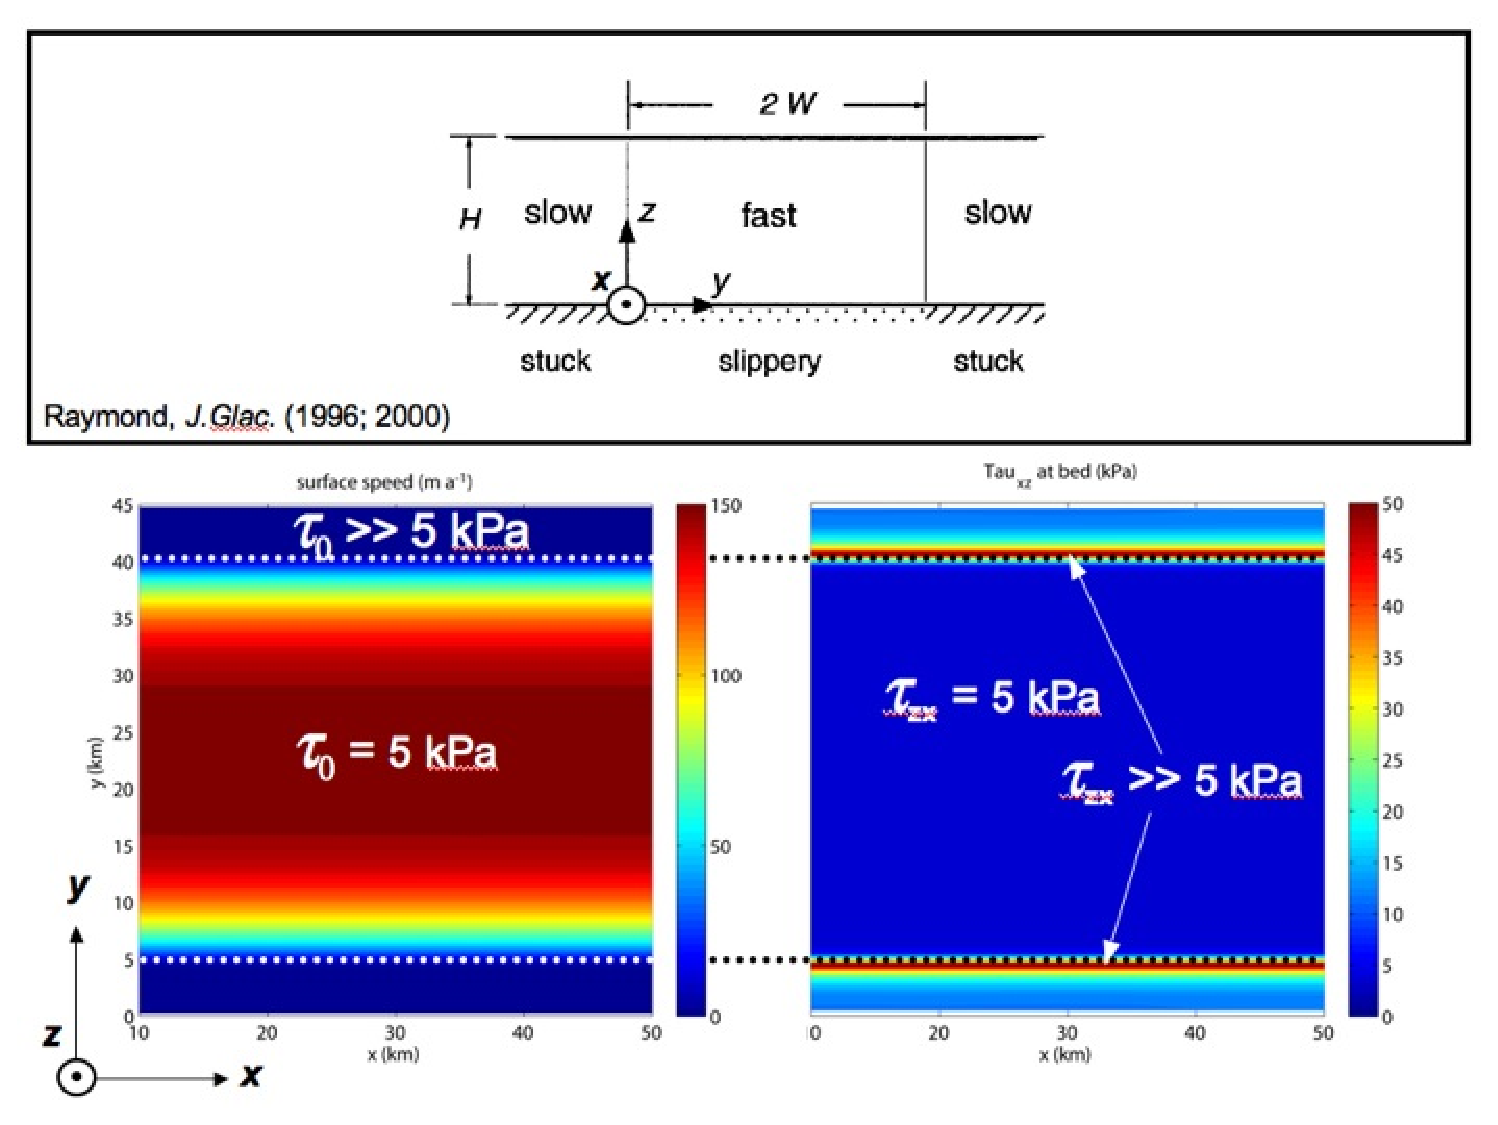
\includegraphics[width=0.65\columnwidth]{\dir/figs/Plastic_bed1.eps}
  \end{center}
  \caption{Idealized ice stream with plastic-bed sliding. Top panel shows a schematic of an idealized ice stream, frozen at the margins and thawed within the ice stream (flow is out of the page). Bottom panel (color) shows a modeled, idealized ice stream (flow is from left to right) with a yield stress of 5 kPa within the ice stream and much larger than 5 kPa outside of it. Bottom left shows the ice stream speed (m/yr) and the bottom right shows the basal drag (kPa). Within the ice stream basal drag is equal to the yield stress. Outside of the ice stream, stress transfer to the lateral margins results in basal drag that is much larger than the yield stress (and also much larger than the driving stress).}
  \label{fig:plasticbed1}
\end{figure} 

%\begin{figure}
%  \begin{center}
%    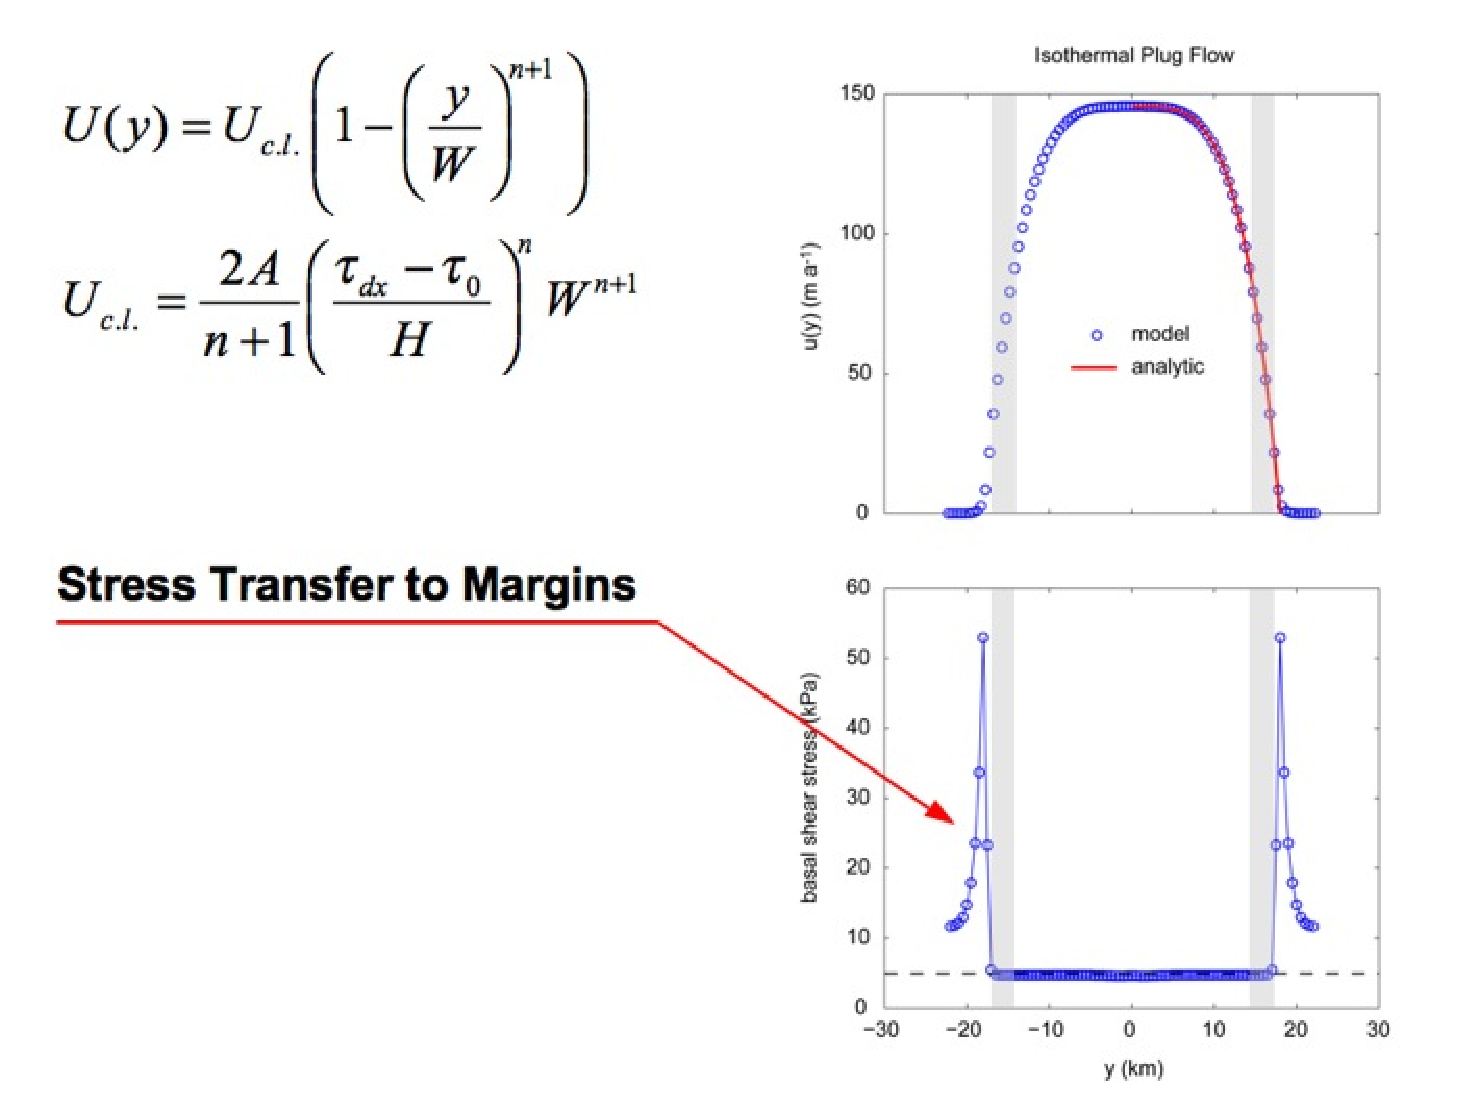
\includegraphics[width=0.65\columnwidth]{\dir/figs/Plastic_bed2.eps}
%  \end{center}
%  \caption{Across-flow profiles of velocity and basal drag from the modeled, idealized ice stream in Figure 1. In the top panel, the analytical solution from \textit{Raymond} (2005) is also shown for comparison. In the bottom panel, stress transfer to the lateral margins is clearly seen.}
%    \label{fig:plasticbed2}
%\end{figure} 

\subsection{Lateral Boundary Conditions}
Currently, the only lateral boundary condition implemented that is of any significance is that for floating ice; the depth-averaged stress resulting from an adjacent column of ocean water is applied at the location of an ice shelf (or ice tongue) front. The derivation follows largely along the lines above for the free surface and specified basal traction boundary conditions, except that the surface normal vectors, $n_{x}$ and $n_{y}$, are taken as lying entirely in the $x$, $y$ plane (that is, they are perpendicular to a vertical shelf front). Thus we have

\begin{equation}
\begin{split}
  & \hat{x}:\quad 4\eta \frac{\partial u}{\partial x}n_{x}+\eta \frac{\partial u}{\partial y}n_{y}+\eta \frac{\partial u}{\partial z}n_{z}=-2\eta \frac{\partial v}{\partial y}n_{x}-\eta \frac{\partial v}{\partial x}n_{y}+\rho g\left( s-z \right)n_{x}-S_{x}, \\ 
 & \hat{y}:\quad 4\eta \frac{\partial v}{\partial y}n_{y}+\eta \frac{\partial v}{\partial x}n_{x}+\eta \frac{\partial v}{\partial z}n_{z}=-2\eta \frac{\partial u}{\partial x}n_{y}-\eta \frac{\partial u}{\partial y}n_{x}+\rho g\left( s-z \right)n_{y}-S_{y} \\ 
\end{split}
\end{equation}

where $S_x$ and $S_y$ are source terms from the pressure due to ocean water (to be defined below) and $\rho g\left( s-z \right)$ comes from including the 1st-order vertical stress balance,

\begin{equation}
\begin{split}
  & \frac{\partial \sigma _{zz}}{\partial z}=\frac{\partial \tau _{zz}}{\partial z}-\frac{\partial P}{\partial z}=\rho g\quad \text{(integrate w}\text{.r}\text{.t}\text{. $z$)}, \\ 
 & P=\rho g\left( s-z \right)+\tau _{zz}, \\ 
 & P=\rho g\left( s-z \right)+2\eta \dot{\varepsilon }_{zz}=\rho g\left( s-z \right)+2\eta \left( -\frac{\partial u}{\partial x}-\frac{\partial v}{\partial y} \right), \\ 
\end{split}
\end{equation}

with \textit{\(\rho{}\)} being the ice density. In the last step above we have used the constitutive relation and incompressibility to expand the vertical, normal-deviatoric stress in terms of the effective viscosity and horizontal-normal strain rates. We calculate the source terms $S_x$ and $S_y$ as the depth-averaged stress at the ice shelf front due to the pressure of ocean water there. This value is given by

\begin{equation}
S_{i}=\left[ \frac{1}{H}\frac{1}{2}\rho _{w}g\left( H-h_f \right)^{2} \right]n_{i}=\left[ \frac{1}{2}\rho _{w}gH\left( \frac{\rho }{\rho _{w}} \right)^{2} \right]n_{i},\quad \quad h_f=H\left( 1-\frac{\rho _{{}}}{\rho _{w}} \right),
\end{equation}

where  \textit{i=x,y}, $n_i$ is the shelf-front normal vector, $H$ is the ice thickness, $h_f$ is the ``freeboard'', or ice thickness above floatation, and $\rho_w$ is the density of ocean water. Because we have taken a depth-average for this source term, we take a depth-average of the term $\rho g\left( s-z \right)$ above, which is $\frac{1}{2}\rho gH$.

Combining these two terms and inserting them in the horizontal boundary condition expressions above gives

\begin{equation}
\begin{split}
& \hat{x}:\quad 4\eta \frac{\partial u}{\partial x}n_{x}+\eta \frac{\partial u}{\partial y}n_{y}+\eta \frac{\partial u}{\partial z}n_{z}= \\
& -2\eta \frac{\partial v}{\partial y}n_{x}-\eta \frac{\partial v}{\partial x}n_{y}+\left[ -\frac{1}{2}H\left( \frac{\rho }{\rho _{w}} \right)^{2}\rho _{w}g+\frac{1}{2}\rho gH \right]n_{x}, \\ 
 & \hat{y}:\quad 4\eta \frac{\partial v}{\partial y}n_{y}+\eta \frac{\partial v}{\partial x}n_{x}+\eta \frac{\partial v}{\partial z}n_{z}= \\
 & -2\eta \frac{\partial u}{\partial x}n_{y}-\eta \frac{\partial u}{\partial y}n_{x}+\left[ -\frac{1}{2}H\left( \frac{\rho }{\rho _{w}} \right)^{2}\rho _{w}g+\frac{1}{2}\rho gH \right]n_{y}, \\ 
\end{split}
\end{equation}

which can be rearranged to

\begin{equation}
\begin{split}
  & \hat{x}:\quad 4\frac{\partial u}{\partial x}n_{x}+\frac{\partial u}{\partial y}n_{y}+\frac{\partial u}{\partial z}n_{z}+2\frac{\partial v}{\partial y}n_{x}+\frac{\partial v}{\partial x}n_{y}=\frac{\rho gH}{2\eta }\left( 1-\frac{\rho }{\rho _{w}} \right)n_{x}, \\ 
 & \hat{y}:\quad 4\frac{\partial v}{\partial y}n_{y}+\frac{\partial v}{\partial x}n_{x}+\frac{\partial v}{\partial z}n_{z}+2\frac{\partial u}{\partial x}n_{y}+\frac{\partial u}{\partial y}n_{x}=\frac{\rho gH}{2\eta }\left( 1-\frac{\rho }{\rho _{w}} \right)n_{y}. \\ 
\end{split}
\end{equation}

For an ice shelf, the surface and basal velocities are equal, in which case the vertical velocity gradient terms are $\sim{0}$, giving the final form of the lateral boundary conditions implemented in the model,

\begin{equation}
\begin{split}
  & \hat{x}:\quad 4\frac{\partial u}{\partial x}n_{x}+\frac{\partial u}{\partial y}n_{y}+2\frac{\partial v}{\partial y}n_{x}+\frac{\partial v}{\partial x}n_{y}=\frac{\rho gH}{2\eta }\left( 1-\frac{\rho }{\rho _{w}} \right)n_{x}, \\ 
 & \hat{y}:\quad 4\frac{\partial v}{\partial y}n_{y}+\frac{\partial v}{\partial x}n_{x}+2\frac{\partial u}{\partial x}n_{y}+\frac{\partial u}{\partial y}n_{x}=\frac{\rho gH}{2\eta }\left( 1-\frac{\rho }{\rho _{w}} \right)n_{y}. \\ 
\end{split}
\end{equation}

\subsection{Summary}
Note that the form for \textit{all} of the boundary conditions above is very similar. In fact, all that differs among the equations for the free surface, the specified basal traction, and the lateral shelf boundary condition is (1) the definition of the normal vectors and (2) the existence and definition of a source term. Here are the \textit{x} direction equations again for the three cases:

\begin{equation}
\begin{split}
  & \hat{x}:\quad 4\frac{\partial u}{\partial x}\frac{\partial s}{\partial x}+ \frac{\partial u}{\partial y}\frac{\partial s}{\partial y}+2 \frac{\partial v}{\partial y}\frac{\partial s}{\partial x}+\frac{\partial v}{\partial x}\frac{\partial s}{\partial y}-\frac{\partial u}{\partial z}=0, \\ 
  & \hat{x}:\quad 4\frac{\partial u}{\partial x}\frac{\partial b}{\partial x}+\frac{\partial u}{\partial y}\frac{\partial b}{\partial y}+2\frac{\partial v}{\partial y}\frac{\partial b}{\partial x}+\frac{\partial v}{\partial x}\frac{\partial b}{\partial y}-\frac{\partial u}{\partial z}=\frac{\tau _{bx}}{\eta }, \\ 
  & \hat{x}:\quad 4\frac{\partial u}{\partial x}n_{x}+\frac{\partial u}{\partial y}n_{y}+2\frac{\partial v}{\partial y}n_{x}+\frac{\partial v}{\partial x}n_{y}=\frac{\rho gH}{2\eta }\left( 1-\frac{\rho }{\rho _{w}} \right)n_{x}. \\
\end{split}
\end{equation}

In the first equation (free surface), the normals are related to the ice sheet surface slope and the source term is zero (which subsequently allows us to divide through by the effective viscosity and remove it from the equations). In the second equation (specified basal traction), the normals are related to the bedrock slopes and the source term is related to the assumed relationship between the basal shear stress and the basal sliding rate. In the last equation, the normals are defined by the shape of the ice-shelf front in map view, the vertical velocity gradient terms are absent, and the source term is related to the pressure from the adjacent column of ocean water.
